\documentclass[11pt]{article}
\usepackage{setspace}
\setstretch{1}
\usepackage{amsmath,amssymb, amsthm}
\usepackage{graphicx}
\usepackage{bm}
\usepackage[hang, flushmargin]{footmisc}
\usepackage[colorlinks=true]{hyperref}
\usepackage[nameinlink]{cleveref}
\usepackage{footnotebackref}
\usepackage{url}
\usepackage{listings}
\usepackage[most]{tcolorbox}
\usepackage{inconsolata}
\usepackage[papersize={8.5in,11in}, margin=1in]{geometry}
\usepackage{float}
\usepackage{caption}
\usepackage{esint}
\usepackage{url}
\usepackage{enumitem}
\usepackage{subfig}
\usepackage{wasysym}
\newcommand{\ilc}{\texttt}
\usepackage{etoolbox}
\usepackage{algorithm}
\usepackage{changepage}
% \usepackage{algorithmic}
\usepackage[noend]{algpseudocode}
\usepackage{tikz}
\usetikzlibrary{matrix,positioning,arrows.meta,arrows}
\patchcmd{\thebibliography}{\section*{\refname}}{}{}{}
% \PassOptionsToPackage{hyphens}{url}\usepackage{hyperref}

\providecommand{\myceil}[1]{\left \lceil #1 \right \rceil }
\providecommand{\myfloor}[1]{\left \lfloor #1 \right \rfloor }


\begin{document}



\title{\textbf{CSDS 455: Homework 4}}

\author{Shaochen (Henry) ZHONG, \ilc{sxz517}}
\date{Due and submitted on 09/07/2020 \\ CSDS 455, Dr. Connamacher}
\maketitle

\section{Problem 1}


\section{Problem 2}

For this question I have consulted:
\begin{itemize}
    \item \url{https://math.stackexchange.com/questions/1805181}
    \item \url{https://math.stackexchange.com/questions/2422069}
    \item \url{https://math.ryerson.ca/~danziger/professor/MTH607/W08/Labs/lab12-soln.html}
    \item \url{https://math.stackexchange.com/questions/3681587}
\end{itemize}

\noindent\textbf{W.T.S. if $G$ is a $k$-regular, bipartite graph that can be decomposed into $r$ factors, then $r$ divides $k$.}
\begin{proof}
Since we know that $G$ can be decomposed into $r$ factors, namely, $G$ is $r$-factorable. We may therefore assume that $G$ has $n$ disjoint $r$-factors for $n \in \mathbb{Z}^+$, and the union of these $r$-factors may yield a graph where all of its vertices have a degree of $nr$. This $nr$-regular graph will be the same graph as $G$ (since it is $G$ to be decomposed into $n$ of $r$-factor subgraphs), this means $G$ is a $nr$-regular graph. Since $G$ is known to be $k-regular$, there must be $k = nr$ and the relationship of $r | k$ is demonstrated.
\end{proof}


\noindent\textbf{W.T.S. If $r$ divides $k$, then $G$ is a $k$-regular, bipartite graph that can be decomposed into $r$ factors.}

\begin{proof}
    \leavevmode\newline


    \begin{adjustwidth}{1cm}{}

    \textbf{Lemma: For $G$ being a $k$-regular bipartite graph, $G$ must have a perfect matching $M_1$}.\newline

    \begin{proof}
        It is because the number of edges connected to each vertex in $G$ is $k$, and for $G$ being a bipartite graph with partition $U$ and $V$, the number of edges associated with set $U$ and $V$ must be $k|U|$ and $k|V|$ respectively. Since every edge is connected from a vertex in $U$ to a vertex in $V$, the total number of edges of from $U$ to $V$ is the same as the number of edges from $V$ to $U$ -- this suggest $k|U| = k|V|$, thus $|U| = |V|$.

        Now we want to show that we may find a matching $M_1$ in $G$ by Hall's theorem, and such matching is also a perfect matching. Assume we have $S \subseteq U$ and let $N(S)$ denotes the neighbors of $S$ in $V$. Since every edges starts from $S$ and ends in $N(S)$, denotes $E(S)$ and $E(N(S))$ to be the edge set of edges connected to $S$ and $N(S)$ respectively. Knowing the total number of edges from $S$ to $V$ (namely, to $N(S)$) is $k|S|$ and the total number of edges from $N(S)$ to $U$ is $k|N(S)|$, there must be $k|N(S)| \geq k|S|$ since edges from $N(S)$ to $U$ includes edges from $S \subseteq U$ to $N(S)$.

        This implies $|S| \leq |N(S)|$, then the Hall's condition is achieved and we have a matching of $M_1$ with $|E(M_1)| = |U|$. Since we have previously proven that $|U| = |V|$, and the union of $U$ and $V$ yields all vertices of $G$; $M_1$ has matched every vertex of $G$ and it is therefore a perfect matching of $G$.\newline
    \end{proof}
\end{adjustwidth}

Now with the lemma proven, by the nature of perfect matching $M_1$ must be a $1$-factor of $G$. We denote $G_1 = G - M_1$. This $G_1$ is a $k-1$-regular graph since every vertex of $G$ has decrease a degree of $1$; and this $G_1$ is still bipartite as deletion of edges will not affect the bipartite property. Refer to the above lemma, this $G_1$, being a $k-1$-regular bipartite graph, must have a perfect matching as well (denotes as $M_2$). Following the induction, we may have $G_2 = G_1 - M_2$, $G_3 = G_2 - M_3$... till $G_r = G_{r-1} - M_r = G - M_1 - M_2 - ... - M_r$ being a $(k-r)$-regular graph.\newline

Since $M_1$, $M_2$, ... , $M_r$ are all $1$-factors of $G$, a union of these $M$s may yield a $r$-factor of $G$ and we have showed $G$ has a $r$-factor. Since we know that $r | k$ for $nr = k$ for $n \in \mathbb{Z}^+$, now we keep removing $r$-factors from this $G_r$ (by removing $r$ number of $1$-factors at each time), there must be a $G_{nr} = \emptyset$ with $n$ number of $r$-factors being removed from $G$. We have showed that for $r | k$, $G$ is a $k$-regular, bipartite graph that can be decomposed into $r$ factors.

\end{proof}






\section{Problem 3}


For this question I consulted \url{https://math.stackexchange.com/questions/520203}. I also borrowed the below visual aid from \textit{Elchanan Solomon} who contributed to the above webpage.



\begin{proof}
\leavevmode\newline

To construct a $k$-regular graph with no prefect matching. For $k$ being even, we can simply construct a complete graph of $k+1$ vertices -- since every vertex is connected to $k$ other vertices, this is a $k$-regular graph -- as the graph has $k+1$ vertices, it has no prefect matching.

For $k$ being odd and $k>1$, we will need help from the below lemma.

    \begin{adjustwidth}{1cm}{}

    \textbf{Lemma - Tutte's Theorem (simplified, one direcons): If a simple graph $G$ has a $1$-factor, then there must be $o(G-S) \leq |S|$ for any $S \subseteq V(G)$; where $o(G-S)$ denotes the number of odd components in graph $G-S$.}\newline

    \begin{proof}
        If $G$ has a $1$-factor $M$, then for every odd component $G_o$ of $G-S$ (for $S \subseteq V(G)$), there must be $o(G-S) \leq |S|$. It is because any $G_o$ cannot have any prefect matching (as perfect matching requires even number of vertices), then there must be a vertex $w$ in each $G_o$ that is connected to a vertex in $S$ (denotes this vertex as $S_w$). And this edge $<w, S_w>$ must be in $M$ as otherwise this $w$ will be unmatched.

        As matching is an one-to-one relationship, $o(G-S)$ number of $w$s must be matched to $o(G-S)$ number of $S_w$s. This implies $o(G-S) \leq |S|.$
    \end{proof}
    \end{adjustwidth}

Now to construct the graph $G$. We start with an initial node $u$ and branch out $k$ edges out of it, thus we have $|N(u)| = k$. Now for each $v \in N(u)$, we branch out $k-1$ edges out of it. Then for each $w \in N(v)$, we make a single vertex $w'$ ($\deta{(q)} = 0$) along side the $w$. After all $w'$s are made under a $v$, we fully connect $w$s with $w'$s and then internaly connect each $w'$ to another $w'$. We do it repreatly for next $v$ until this is done to all $v \in N(u)$.\newline

\begin{figure}[H]
    \centering
    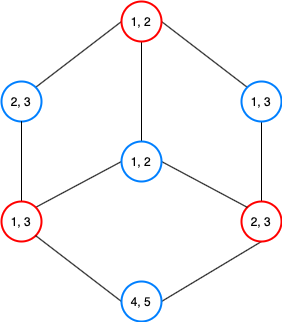
\includegraphics[width=0.7\linewidth]{{fig/fig_p3.png}}
    \caption{Demo of $G$ for $k = 5$ (modified work based on Elchanan Solomon's diagram)}
    \label{fig:1}
\end{figure}

This $G$ will be a $k$-regular graph because: $u$ branch out for $k$ edges, $\delta{(u)} = k$; every $v$ branch out $k-1$ edges and connected to $u$, therefore $\forall \delta{(v)} = k$; every $w$ is connected to $k-1$ number of $w'$ and also to a $v$, so $\forall \delta{(w)} = k$; finally, every $w'$ is connected to $k-1$ number of $w$ and also to another $w'$, therefore $\forall \delta{(w')} = k$.\newline

Now if we let this $u$ to be $S$, and for $G-S$ we have all $k$ compoments left. All of these components (lead by $v \in N(u)$) are odd components, as:

\begin{equation}
    k-1 + k-1 + 1 = 2k-1
\end{equation}

For $k$ being odd, $2k-1$ must be odd. This voids the above lemma since the contrapositive of lemma ``\textit{$G$ has a $1$-factor $\longrightarrow$ $o(G-S) \leq |S|$ for any $S \subseteq V(G)$}'' is  ``\textit{$o(G-S) > |S|$ for any $S \subseteq V(G)$ $\longrightarrow$ $G$ has a no $1$-factor}.''

Now we have $|S| = 1$ but $o(G-S) = k$ (known that $k > 1$), thus $G$ has no $1$-factor and therefore has no perfect matching. \newline

We have demonstrated there is a way to construct a $k$-regular graph $G$ for both $k$ being even and odd (for $k>1$), thus there is a way to construct such graph $G$ for all $k > 1$ for $k \in \mathbb{Z}^+$.

\end{proof}

% \section{References}
%
% \nocite{*}
% \raggedright
% \bibliography{references.bib}
% \bibliographystyle{plain}


\end{document}